%! TeX program = lualatex
%---------------------------ALLGEMEINE IMPORTS-------------------------------------
\documentclass[12pt,english,ngerman]{scrartcl}

\input{./input/shared_preamble.tex}

\addbibresource{cmos.bib}
    % Kopfzeile
\ihead{SS22\\18.05.2022}
\chead{\textsc{Hinterleitner} Michael - 12002411 \\ \textsc{Philipp} Maximilian - 11839611}
\ohead{LU ECM-\\ CMOS Logik}
    % Fußzeile
%--------------------------------------AB HIER DOKUMENT---------------------------------------------
\begin{document}
% \includepdf{deckblatt2.pdf}
\tableofcontents
\newpage


%\section{Aufgabenstellung}\label{sec:Aufgabenstellung}

% Die nachfolgende Aufgabenstellung wurde von den Laborbetreuern bereitgestellt
% und beinhaltet sowohl Angaben zur Vorbereitung als auch zur praktischen
% Durchführung der Übung:

% zu 1: Aufgabenstellung Das vor der Übung verteilte Aufgabenblatt.
 \includepdf[
     pages=-,  % all pages
     addtotoc={
         1, section, 1, Aufgabenstellung, sec:Aufgabenstellung
     }
 ]{angabe.pdf}

% zu 2: Vorbereitung Es sind beide Vorbereitungen dem Protokoll beizufügen.
% \section{Vorbereitung}\label{sec:Vorbereitung}
%Die folgende Vorbereitung wurde vor der Laborübung 
\includepdf[pages=-,
     addtotoc={
         1, section, 2, Vorbereitung, sec:Vorbereitung
     }]{./figures/CMOS-Logik1.pdf}
\includepdf[pages=-]{./figures/CMOS-Logik2.pdf}
% \includepdf[pages=-]{./mh_vorbereitung_opv.pdf}


% zu 3: Grundlagen In den Grundlagen sollen die später verwendeten Formeln
% stehen und kurz erklärt werden, dabei ist es nicht notwendig Formeln
% herzuleiten. Quellenangaben sind an dieser Stelle von Vorteil, weil Sie so
% schnell die betreffenden Stellen in Unterlagen finden. In den Rechnungen
% werden grundlegende Annahmen skizziert und begründet und dann mit diesen
% Annahmen, die für die Schaltungen notwendigen Werte berechnet. Dabei kann
% auch gleich auf die später wirklich verwendeten Werte Bezug genommen werden -
% wir verwenden bei den Widerständen zum Beispiel von den Normwert-Reihen die
% E12 und/oder E24 Serie (nach DIN 41426 bzw. IEC 63).
\section{Grundlagen}\label{sec:Grundlagen}
%in Grundlagen
Operationsverstärker (kurz 'OPV oder 'OpAmp') dienen der Verstärkung von
Gleichspannungen. Sie besitzen einen nicht-invertierenden, der meist mit einem
Plus gekennzeichnet ist, und einen invertierenden Eingang, der häufigst mit
einem Minus dargestellt wird. Zu beachten ist, dass die Verstärkung auf die
Differenzspannung der beiden Eingänge wirkt. Je zwei zusätzliche Anschlüsse
finden sich für die positive und negative Betriebsspannung und für den
Offsetabgleich, damit bei keiner Eingangsspannung auch keine Ausgangsspannung
auftritt - dieser wird also in einer externen Schaltung durchgeführt.
%In \autoref{fig:pin_anschl} sind die Pins eines Operationsverstärkers, wie er
%auch in der Laborübung verwendet wurde, zu sehen.


Es gibt vier grundlegende Arten der Verwendung von Operationsverstärkern,
darunter der nicht-invertierende Betrieb, bei dem das Eingangssignal nur auf
den nicht-invertierenden Kanal gelegt wird und der invertierende auf Masse
gelegt wird. Analog funktioniert der invertierende Modus, bei dem das Signal
nun an den invertierenden Eingang gelegt wird, wodurch die Ausgangsspannung
zusätzlich zur Verstärkung noch zum Eingangssignal invertiert wird. Beim
Differenzbetrieb werden an beide Eingänge Signale angelegt und die
Differenzspannung verstärkt. Im Falle des Gleichtaktbetriebs liegt das gleiche
Eingangssignal an den beiden Eingängen an, wodurch es theoretisch keine
Differenzspannung und Verstärkung geben sollte - in der Realität resultiert
allerdings eine Verstärkung, die als Gleichtkatkverstärkung bezeichnet wird.

Da der Operationsverstärker ohne zusätzliche Verkopplung sehr stark
frequenzabhängig ist und nur eine geringe Bandbreite gewünscht verstärkt, wird
eine Gegenkopplung vom Ausgang zum Eingang durchgeführt, wodurch die
Verstärkung zwar abnimmt, die Bandbreite jedoch stark vergrößert wird. Die
Bandbreite wird wie gewohnt durch die Grenzfrequenz chraktersisiert, bei
welcher die Verstärkung noch \SI{70}{\%} der maximalen beträgt.

Die resultierende Verstärkung lässt sich gemäß \autoref{eq:ver} als Verhätlnis
der Eingangs- $U_e$ zur Ausgangsspannung $U_a$ berechnen.
%insert eq ---


%in Durchführung
Zu beachten ist, dass jeder nicht belegte Pin auf Massenpotential gelegt wird.


% zu 4: Versuchsdurchführung In diesem Punkt wird die Durchführung der
% einzelnen Aufgaben beschrieben. Im Simulationsteil ist die simulierte
% Schaltung mit allen Analyseparametern darzustellen. Im praktischen Teil sind
% die verwendete Geräte sowie die gemessenen Werte der verwendeten Bauteile
% anzugeben. Außerdem sind durchgeführte Funktionsüberprüfungen der Bauteile
% (Dioden, Transistor, etc.) anzuführen. Die Messergebnisse bzw. Oszillogramme
% sind mit Angabe der verwendeten Messgeräte anzugeben. Oszillogramme werden
% vom verwendeten Oszilloskop als Daten auf einen USB-Stick ausgegeben und
% können in das Protokoll aufgenommen werden. Das gleiche gilt für Schaltungen
% bzw. Ergebnissen von Simulationen. Es ist auf eine klare Darstellung der
% Messergebnisse und –auswertung zu achten (Tabellen, geeignete Grafiken). Die
% originalen, während des Versuchs angefertigten Aufzeichnungen sind dem
% Protokoll beizufügen. 
\section{Versuchsdurchführung}\label{sec:versuchsdurchfuehrung}
Für den praktischen Teil an der Steckplatine wurden Widerstände der E12-Reihe,
mit denen die in der Vorbereitung angegebenen respektive errechneten Werte
angenähert wurden, verwendet. 

Die verwendeten Geräte sind \autoref{tab:geraeteliste} zu entnehmen.

\begin{table}
  \caption{Tabelle der verwendeten Geräte}
  \label{tab:geraeteliste}
  \centering
  \begin{tabular}{l|l}
    \hline
   \multicolumn{2}{ c }{\textbf{Geräteliste}} \\
    \hline
    \textbf{Gerät/Bauelement} & \textbf{Typ} \\
    \hline
    Oszilloskop & \textit{Tektronix TDS 2002}\cite{oszilloscope}\\
    Funktionsgenerator & \textit{H-TRONIC FG250D}\cite{funktionsgenerator} \\
    Netzgerät & nicht bestimmbar\\
    Multimeter & \textit{Fluke 175 TrueRMS}\cite{fluke175} \\
    % todo references
    N-MOSFET & \textit{ZVN2106A}\\
    P-MOSFET & \textit{ZVP2106A}\\
    NOT-Gatter & \textit{74LS04}\\
    2x-NOR-Gatter & \textit{74LS02}\\
    3x-NOR-Gatter & \textit{74LS27}\\
    \hline
  \end{tabular}
\end{table}

\paragraph{Entprellter Schalter}
%TODO text erklaeren wie der Schalter angesteuert wird und wo er verwendet wurde
Der entprellter Schalter wird als Signalgeber für die logischen Schaltungen und
Gatter verwendet. Der Aufbau dieses Schalters ist in
\autoref{fig:aufbau_schalter} ersichtlich, jedoch ist noch der \textit{GND} mit
Ground und \textit{VCC} mit \SI{5}{\volt} zu beschalten damit das Signal von
Schalter eins bzw Schalter zwei von den jeweiligen Betriebsart abgegriffen
werden.

Jeder dieser Schalter hat einen Standard \textit{HIGH} bzw.
\textit{LOW} Betriebsart.

\begin{figure}[H]
  \centering
    % \includegraphics[width=0.95\textwidth]{./figures/messungen/schalter.png}
  \caption{}
  \label{fig:aufbau_schalter}
\end{figure}


\paragraph{LED Leiste}
%TODO text erklaeren wie der Leiste angesteuert wird und wo er verwendet wurde
Damit die Eingangssignale und Ausgangssignale der logischen Schaltungen
dargestellt werden kann, wird eine LED-Leiste verwendet. Diese besteht aus
mehreren LEDs mit Vorwiderständen und ist in \autoref{fig:aufbau_led} dargestellt und
unterstützt bis zu 8 Aus- bzw Eingangssignale. Die hier verwendete LED-Leiste
hat einen Common-Ground und somit werden positiven Spannungssignale direkt an den
verschiedenen Anschlüssen angelegt um die LED zum Leuchten zu bringen.

\begin{figure}[H]
  \centering
    % \includegraphics[width=0.95\textwidth]{./figures/messungen/schalter.png}
  \caption{}
  \label{fig:aufbau_led}
\end{figure}

Damit die Aufnahmen der Schaltungen übersichtlich bleiben wurde diese meistens
von den Aufnahmen weggeschnitten und in der Grafik mittels \textit{LED} oder in
der Beschriftung gekennzeichnet bzw. erwähnt.

\subsection{CMOS}
% Simulation:
\subsubsection{Simulation}
% 2.1
% Die Inverter-Schaltung ist mit LTspice zu simulieren.
\paragraph{Aufbau des CMOS-Inverters}

%TODO text simulation

%TODO figure sim Aufbau
\begin{figure}[H]
  \centering
    % 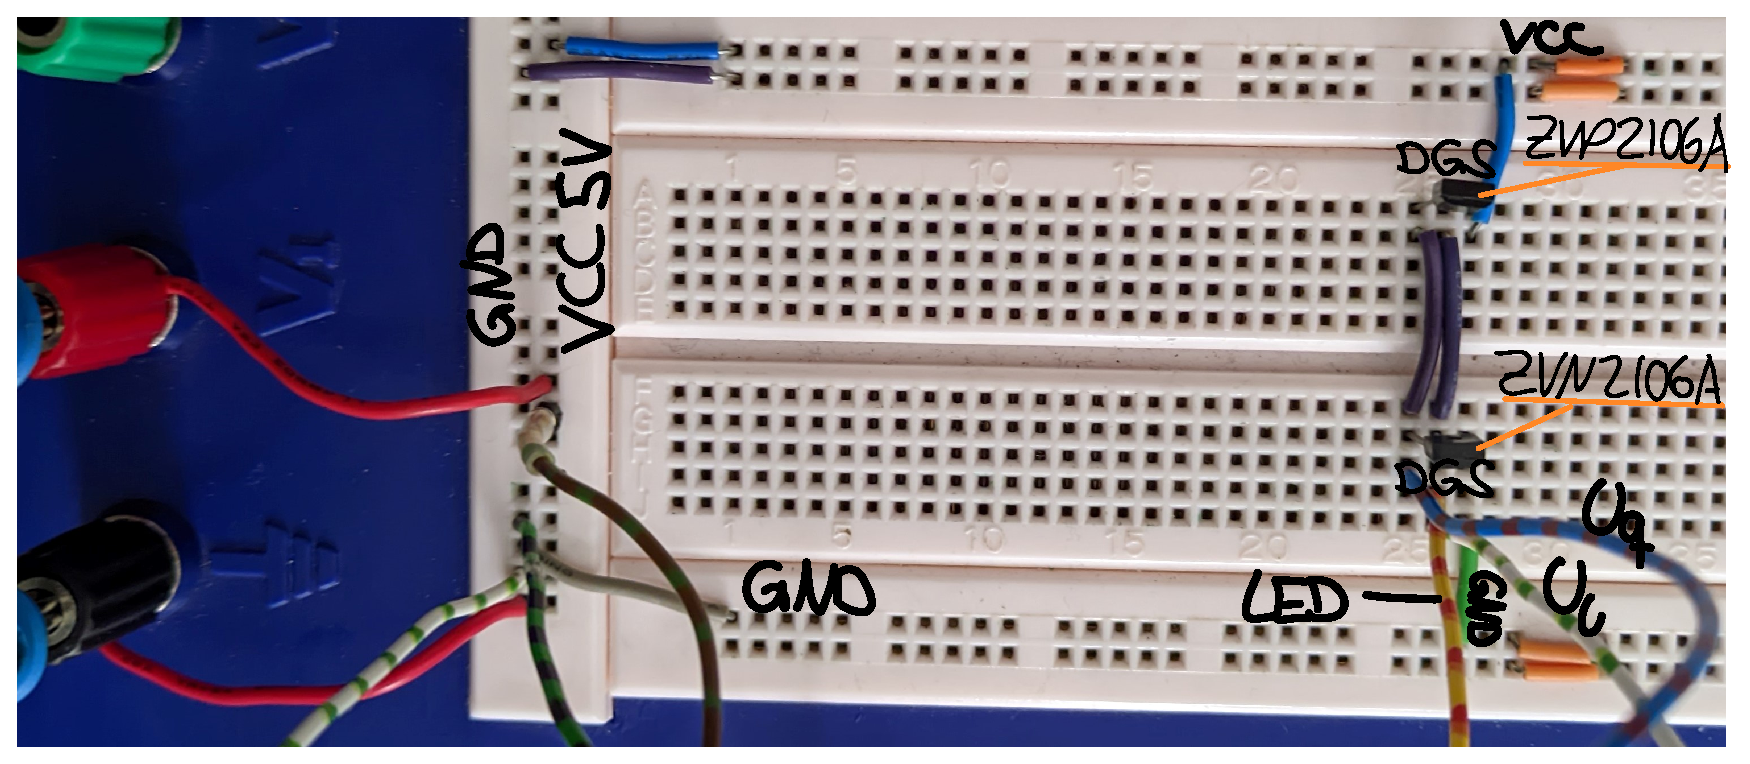
\includegraphics[width=0.95\textwidth]{./figures/messungen/aufbauinverter.pdf}
  \caption{}
  \label{fig:sim_aufbau_inv}
\end{figure}


% Die Übertragungskennlinie
% und die Stromaufnahme sind darzustellen (PULSE-Quelle).
%TODO text messung Wie wurde simuliert wie wurde die Schwellspannung gemessen.

%TODO figure messung
% 2.2
% Die Gate-Source Schwellspannung ist mit jener der Datenblätter zu vergleichen.

% 2.3
% Die Schaltung des  NAND-Gatters ist mit LTspice zu simulieren. Die Ein- und
% Ausgangsspannungen sind darzustellen (PULSE-Quelle).
\paragraph{Aufbau des CMOS-NAND-Gatters}
%TODO text sim aufbau

%TODO figure sim aufbau
\begin{figure}[H]
  \centering
    % 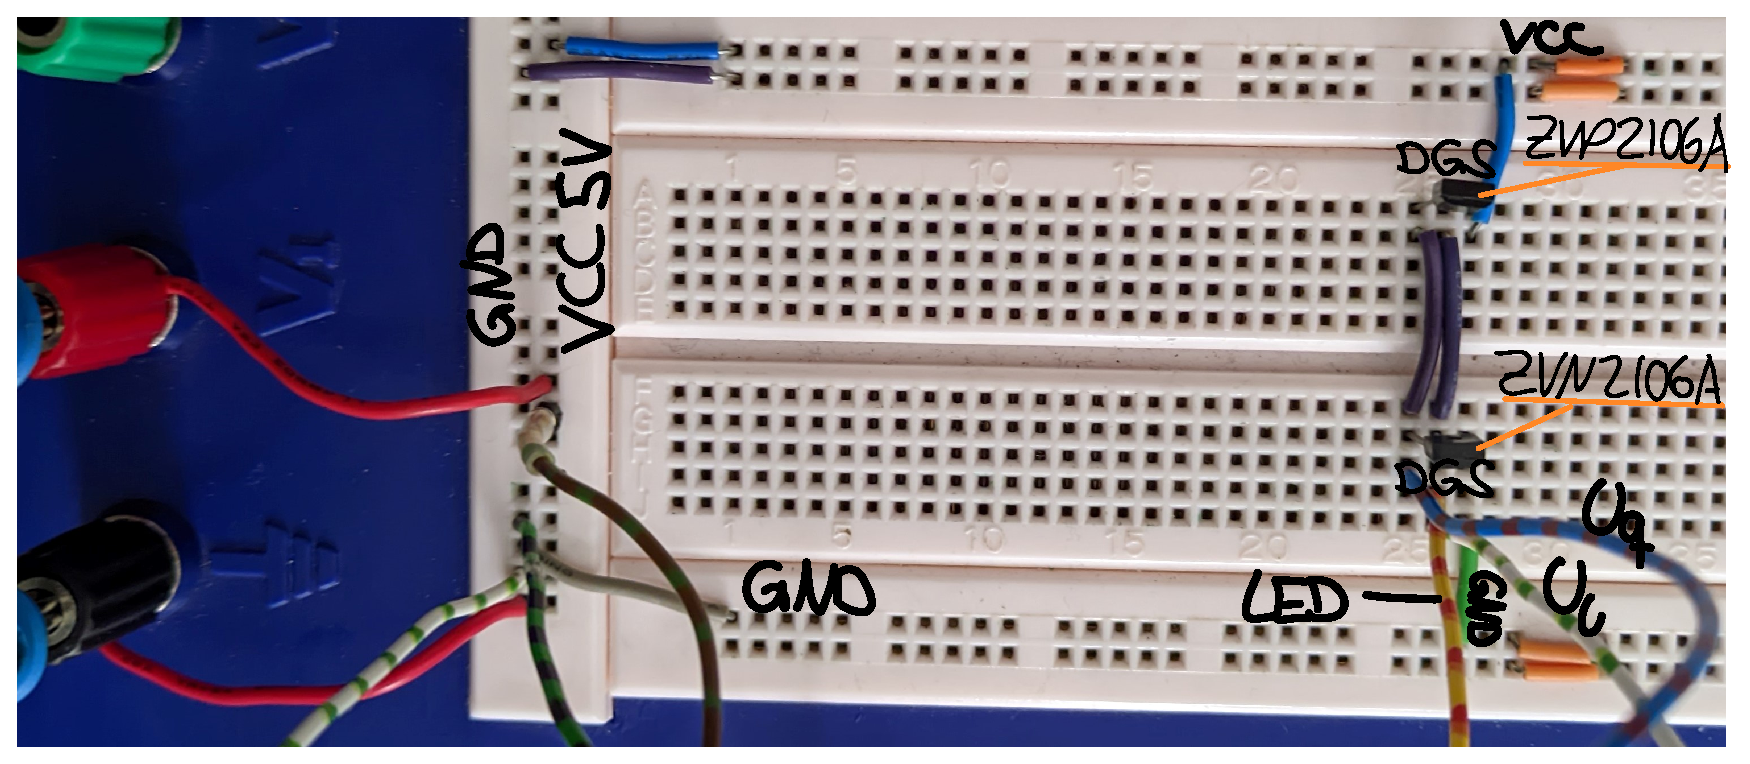
\includegraphics[width=0.95\textwidth]{./figures/messungen/aufbauinverter.pdf}
  \caption{}
  \label{fig:sim_aufbau_nand}
\end{figure}

%TODO text messung Wie wurde die verschiedenen logic states geschalten

%TODO figure messung

% Aufbau am Steckboard:
\subsubsection{Steckboard}
% 2.4 Der CMOS-Inverter ist auf dem Steckboard aufzubauen und seine
% Funktionalität zu prüfen. 
\paragraph{Aufbau des CMOS-Inverters}\label{sec:mess_cmos}
%TODO text
Zunächst wird der CMOS-Inverter mittels zweier MOSFETs (einem PMOS \cite{} und
einem NMOS \cite{}) wie nach dem Schaltbild (\autoref{fig:sim_aufbau_inv})
aufgebaut. Jedoch wurden zur Visualisierung des Eingangszustands $U_l$ und des
Ausgangszustands $U_q$ LEDs der LED-Leiste parallel dazu geschaltet. Das
Eingangssignal wurde durch einen entprellten Schalter, im Standardzustand
\textit{LOW}, gegeben, der Aufbau genaue kann im \autoref{} gesehen werden. Als
Spannungsquelle wurde einstellbares Netzteil verwendet und auf \SI{5}{\volt}
eingestellt. 

%TODO figure
\begin{figure}[H]
  \centering
    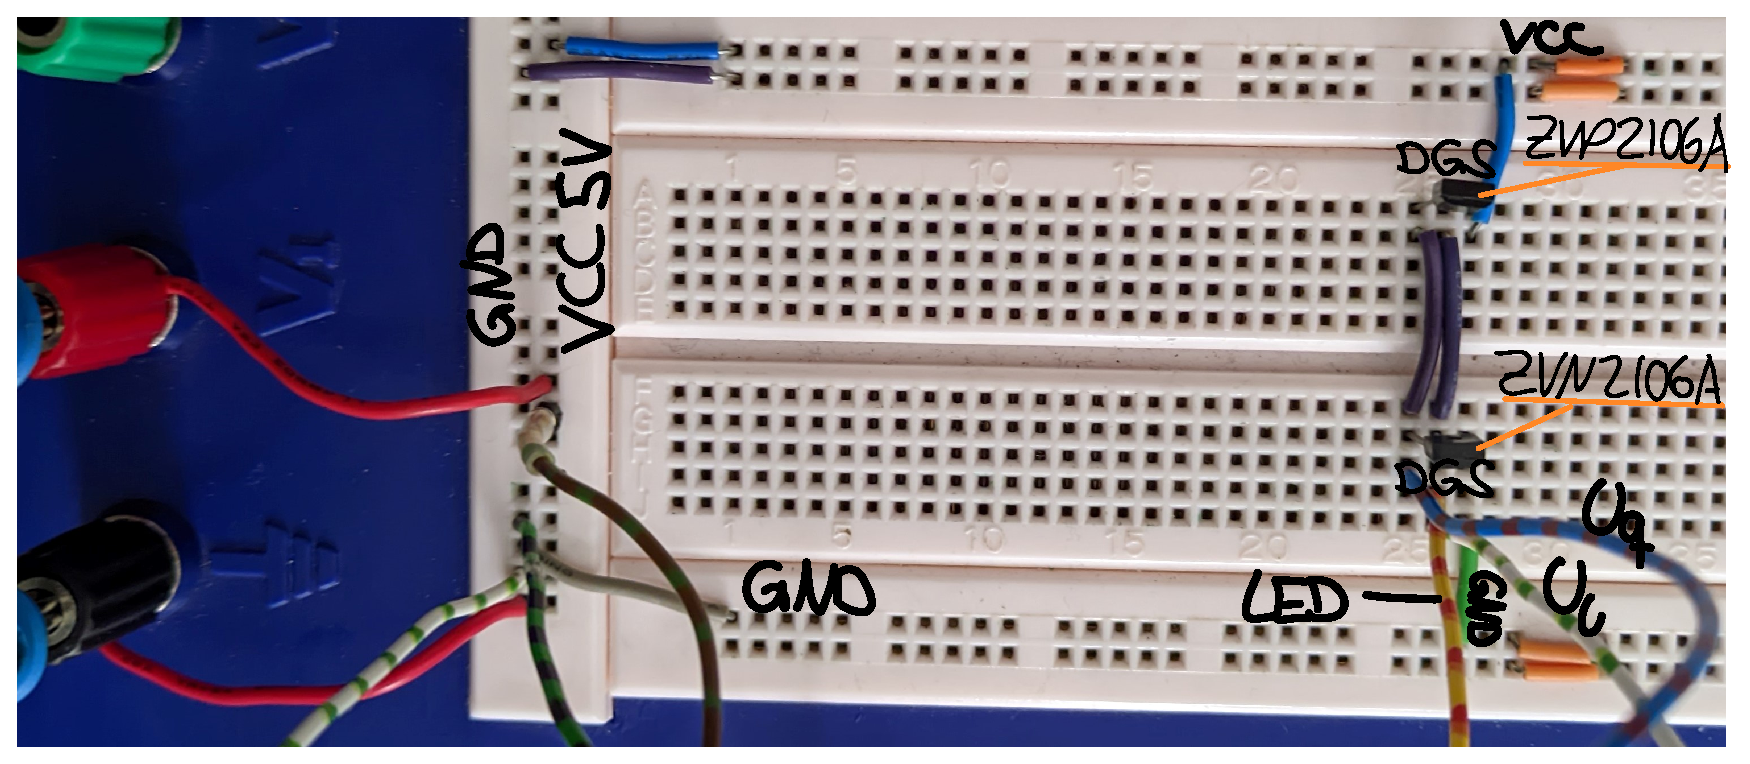
\includegraphics[width=0.95\textwidth]{./figures/messungen/aufbauinverter.pdf}
  \caption{Dies ist der Aufbau einer CMOS-Inverter-Schaltung nach dem
  Schaltplan aus \autoref{fig:sim_aufbau_inv}. Wobei $U_q$ das Ausgangssignal
  der Schaltung ist  und $U_l$ das logische Eingangssignal ist. Der Zustand
  beider kann anhand einer LED in der LED-Leiste abgelesen werden.}
  \label{fig:mess_aufbau_inv}
\end{figure}


Um die Funktionstüchtigkeit des CMOS-Gatters zu überprüfen wurde die
Wahrheitstafel des NOT-Gatters im Eingang durch geschaltet die gemessenen Werte
sind in \autoref{fig:mess_wahrheitstabelle_inv} ersichtlich.
%TODO text messung
% Als  Pegelgeber wird  für  das  Steckboard  ein vorhandener  elektronisch
% entprellte  Schalter  (mit  Hilfe  eines RS-Flip-Flops)  verwendet.  Der
% Ein-  und Ausgangszustand  ist  jeweils durch  LEDs  anzuzeigen.  Die
% Funktionalität  der Schaltung ist anhand der LEDs zu zeigen.
%TODO figure messung

\begin{figure}[H]
  \centering
    \includegraphics[width=0.95\textwidth]{./figures/messungen/WahrheitstabelleInverter.pdf}
  \caption{}
  \label{fig:mess_wahrheitstabelle_inv}
\end{figure}


% 2.5
% Die Schaltung des  NAND-Gatters ist auf dem Steckboard aufzubauen und ihre
% Funktionalität anhand der LEDs zu zeigen.
\paragraph{Aufbau des CMOS-NAND-Gatters}
%TODO text
Nun ist CMOS-NOT Schaltung um zwei weiter MOSFETs erweitert worden, um ein
NAND-Gatter zu bauen. Dies wurde wie in \autoref{fig:sim_aufbau_nand} gemacht,
jedoch wurde wie auch im \nameref{sec:mess_cmos} entprellte Schalter als
Pegelgeber und die LED-Leiste zur Visualisierung der Pegel(Signale) verwendet.
Diese wurden ebenfalls an den geeigneten Stellen angeschlossen, wie diese genau
angeschlossen wurden ist der \autoref{fig:mess_aufbau_nand} entnehmbar.

%TODO figure
\begin{figure}[H]
  \centering
    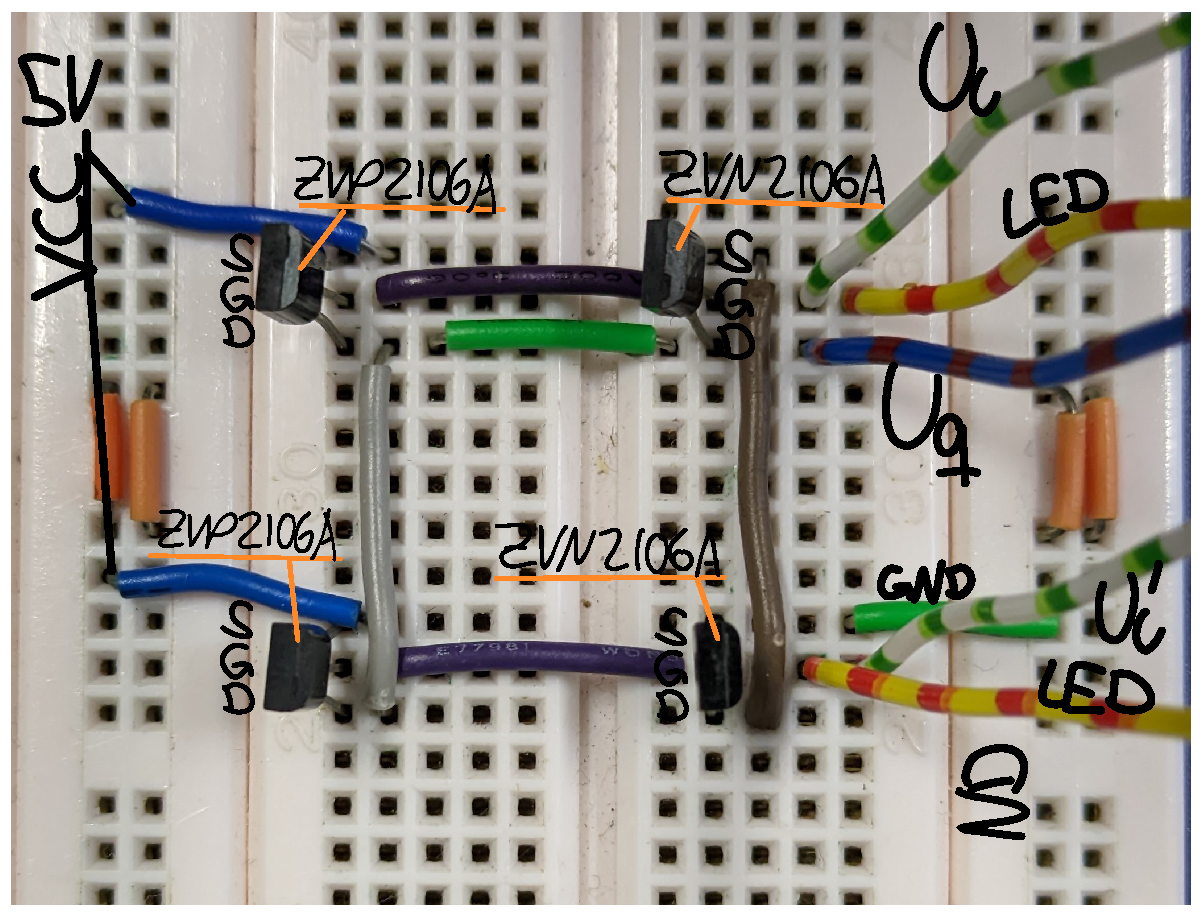
\includegraphics[width=0.95\textwidth]{./figures/messungen/aufbaunand.pdf}
  \caption{Dies ist der Aufbau eines CMOS-NAND-Gatters nach dem Schaltplan aus \autoref{fig:sim_aufbau_nand}}
  \label{fig:mess_aufbau_nand}
\end{figure}

%TODO text messung
Um die Funktionstüchtigkeit des CMOS-Gatters zu überprüfen wurde die
Wahrheitstafel des NAND-Gatters in den zwei Eingängen ($U_l$ $U_l'$) durch
geschaltet die gemessenen Werte sind in \autoref{fig:mess_wahrheitstabelle_nand}
ersichtlich.


%TODO figure messung
\begin{figure}[H]
  \centering
    \includegraphics[width=0.95\textwidth]{./figures/messungen/WahrheitstabelleNAND.pdf}
  \caption{}
  \label{fig:mess_wahrheitstabelle_nand}
\end{figure}

% 2.6
% Die Ergebnisse sind zu protokollieren und diskutieren.

\subsection{Schaltungssynthese}
% Simulation:
% 2.1 Die Schaltung ist mit LTspice zu simulieren.
\subsubsection{Simulation}

%TODO text sim aufbau

%TODO figure sim aufbau
\begin{figure}[H]
  \centering
    % 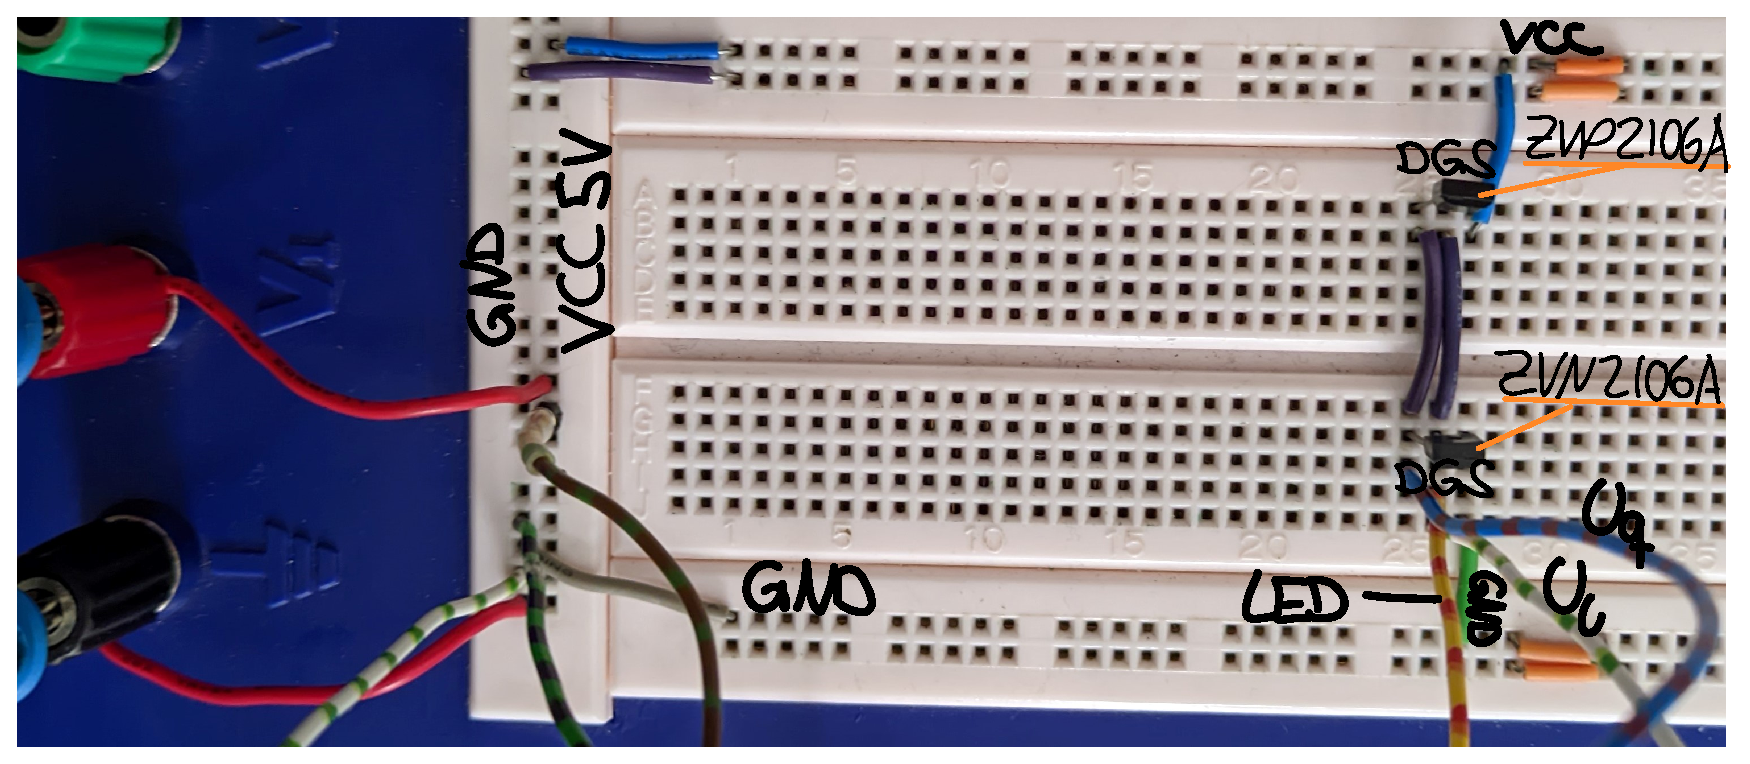
\includegraphics[width=0.95\textwidth]{./figures/messungen/aufbauinverter.pdf}
  \caption{}
  \label{fig:sim_aufbau_alarm}
\end{figure}

% Die Eingangsspannungen, für die geeignete Perioden zu definieren sind, sowie
% die Ausgangsspannung sind darzustellen.
%TODO text messung Wie wurde die verschiedenen logic states geschalten

%TODO figure messung


% Aufbau am Steckboard:
\subsubsection{Steckboard}
Wie \nameref{sec:Aufgabenstellung} 

%TODO text

%TODO figure
\begin{figure}[H]
  \centering
    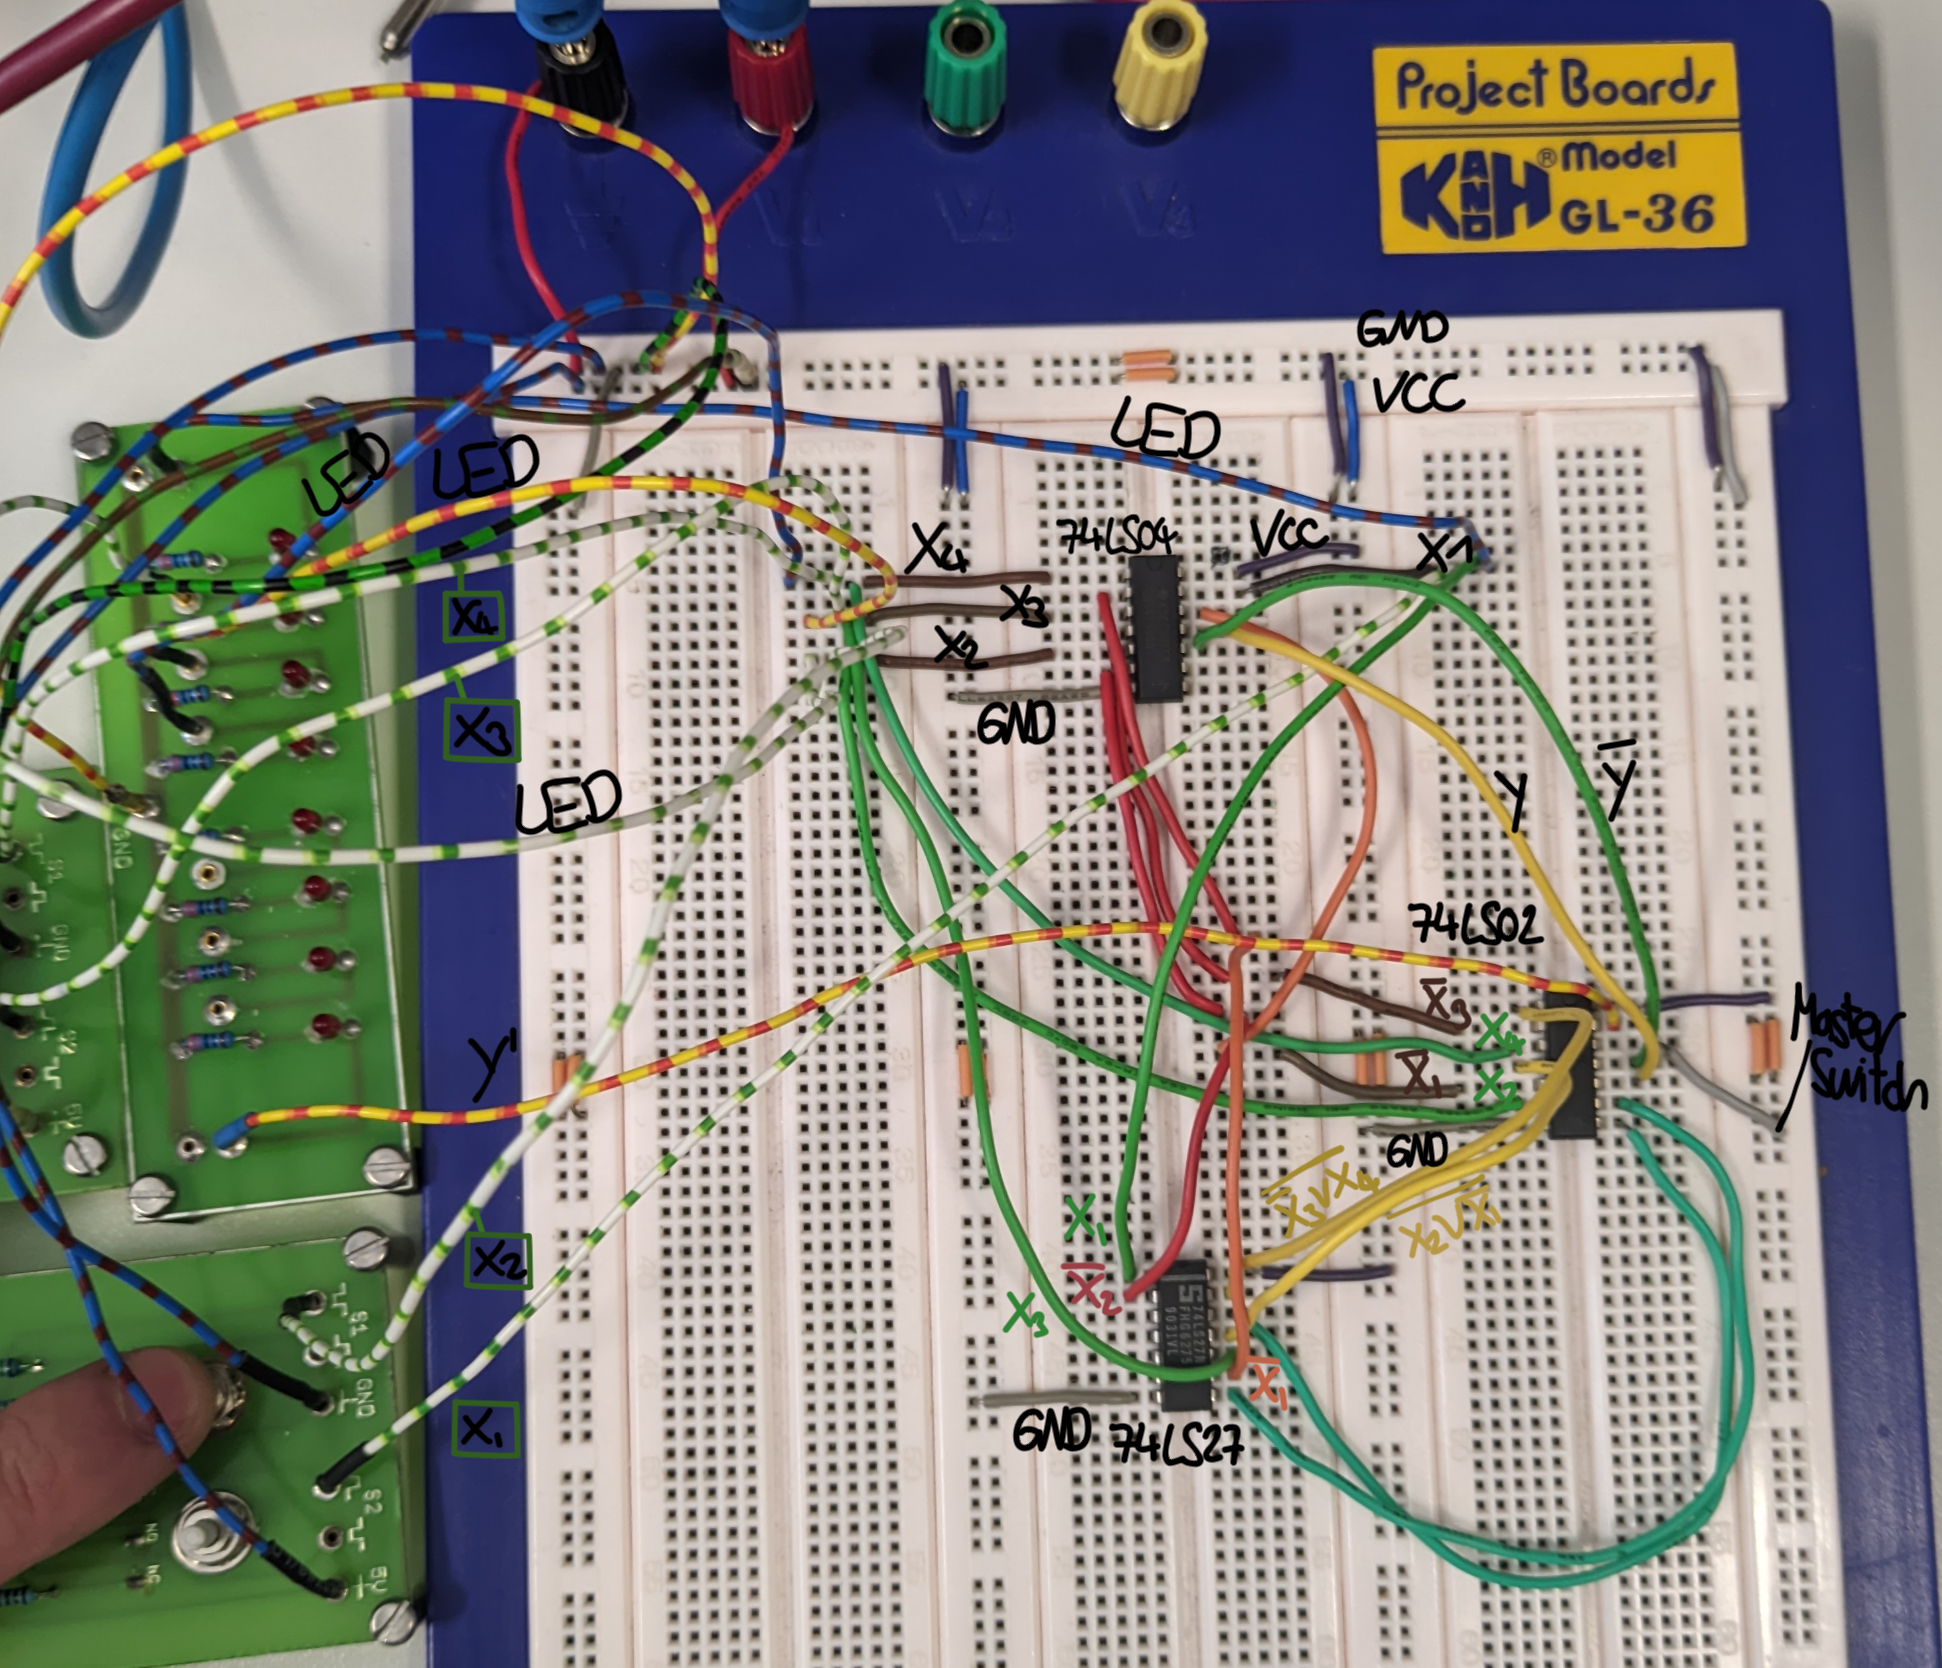
\includegraphics[width=0.95\textwidth]{./figures/messungen/aufbaualarm.png}
  \caption{Dies ist der Aufbau der Einbruchsicherungsschaltung nach dem
  Schaltplan aus \autoref{fig:sim_aufbau_alarm}}
  \label{fig:mess_aufbau_alarm}
\end{figure}

% 2.2
% Die Schaltung ist am Steckboard aufzubauen und ihre Funktionalität an Hand der 
% Wahrheitstafel zu zeigen. Als Pegelgeber werden für das Steckboard vorhandene 
% elektronisch entprellte Schalter verwendet. Die logischen Zustände von x1, x2, x3, 
% x4 und y, sowie des Master-Switch, sind durch LEDs anzuzeigen.
%TODO text messung

%TODO figure messung
\begin{figure}[H]
  \centering
    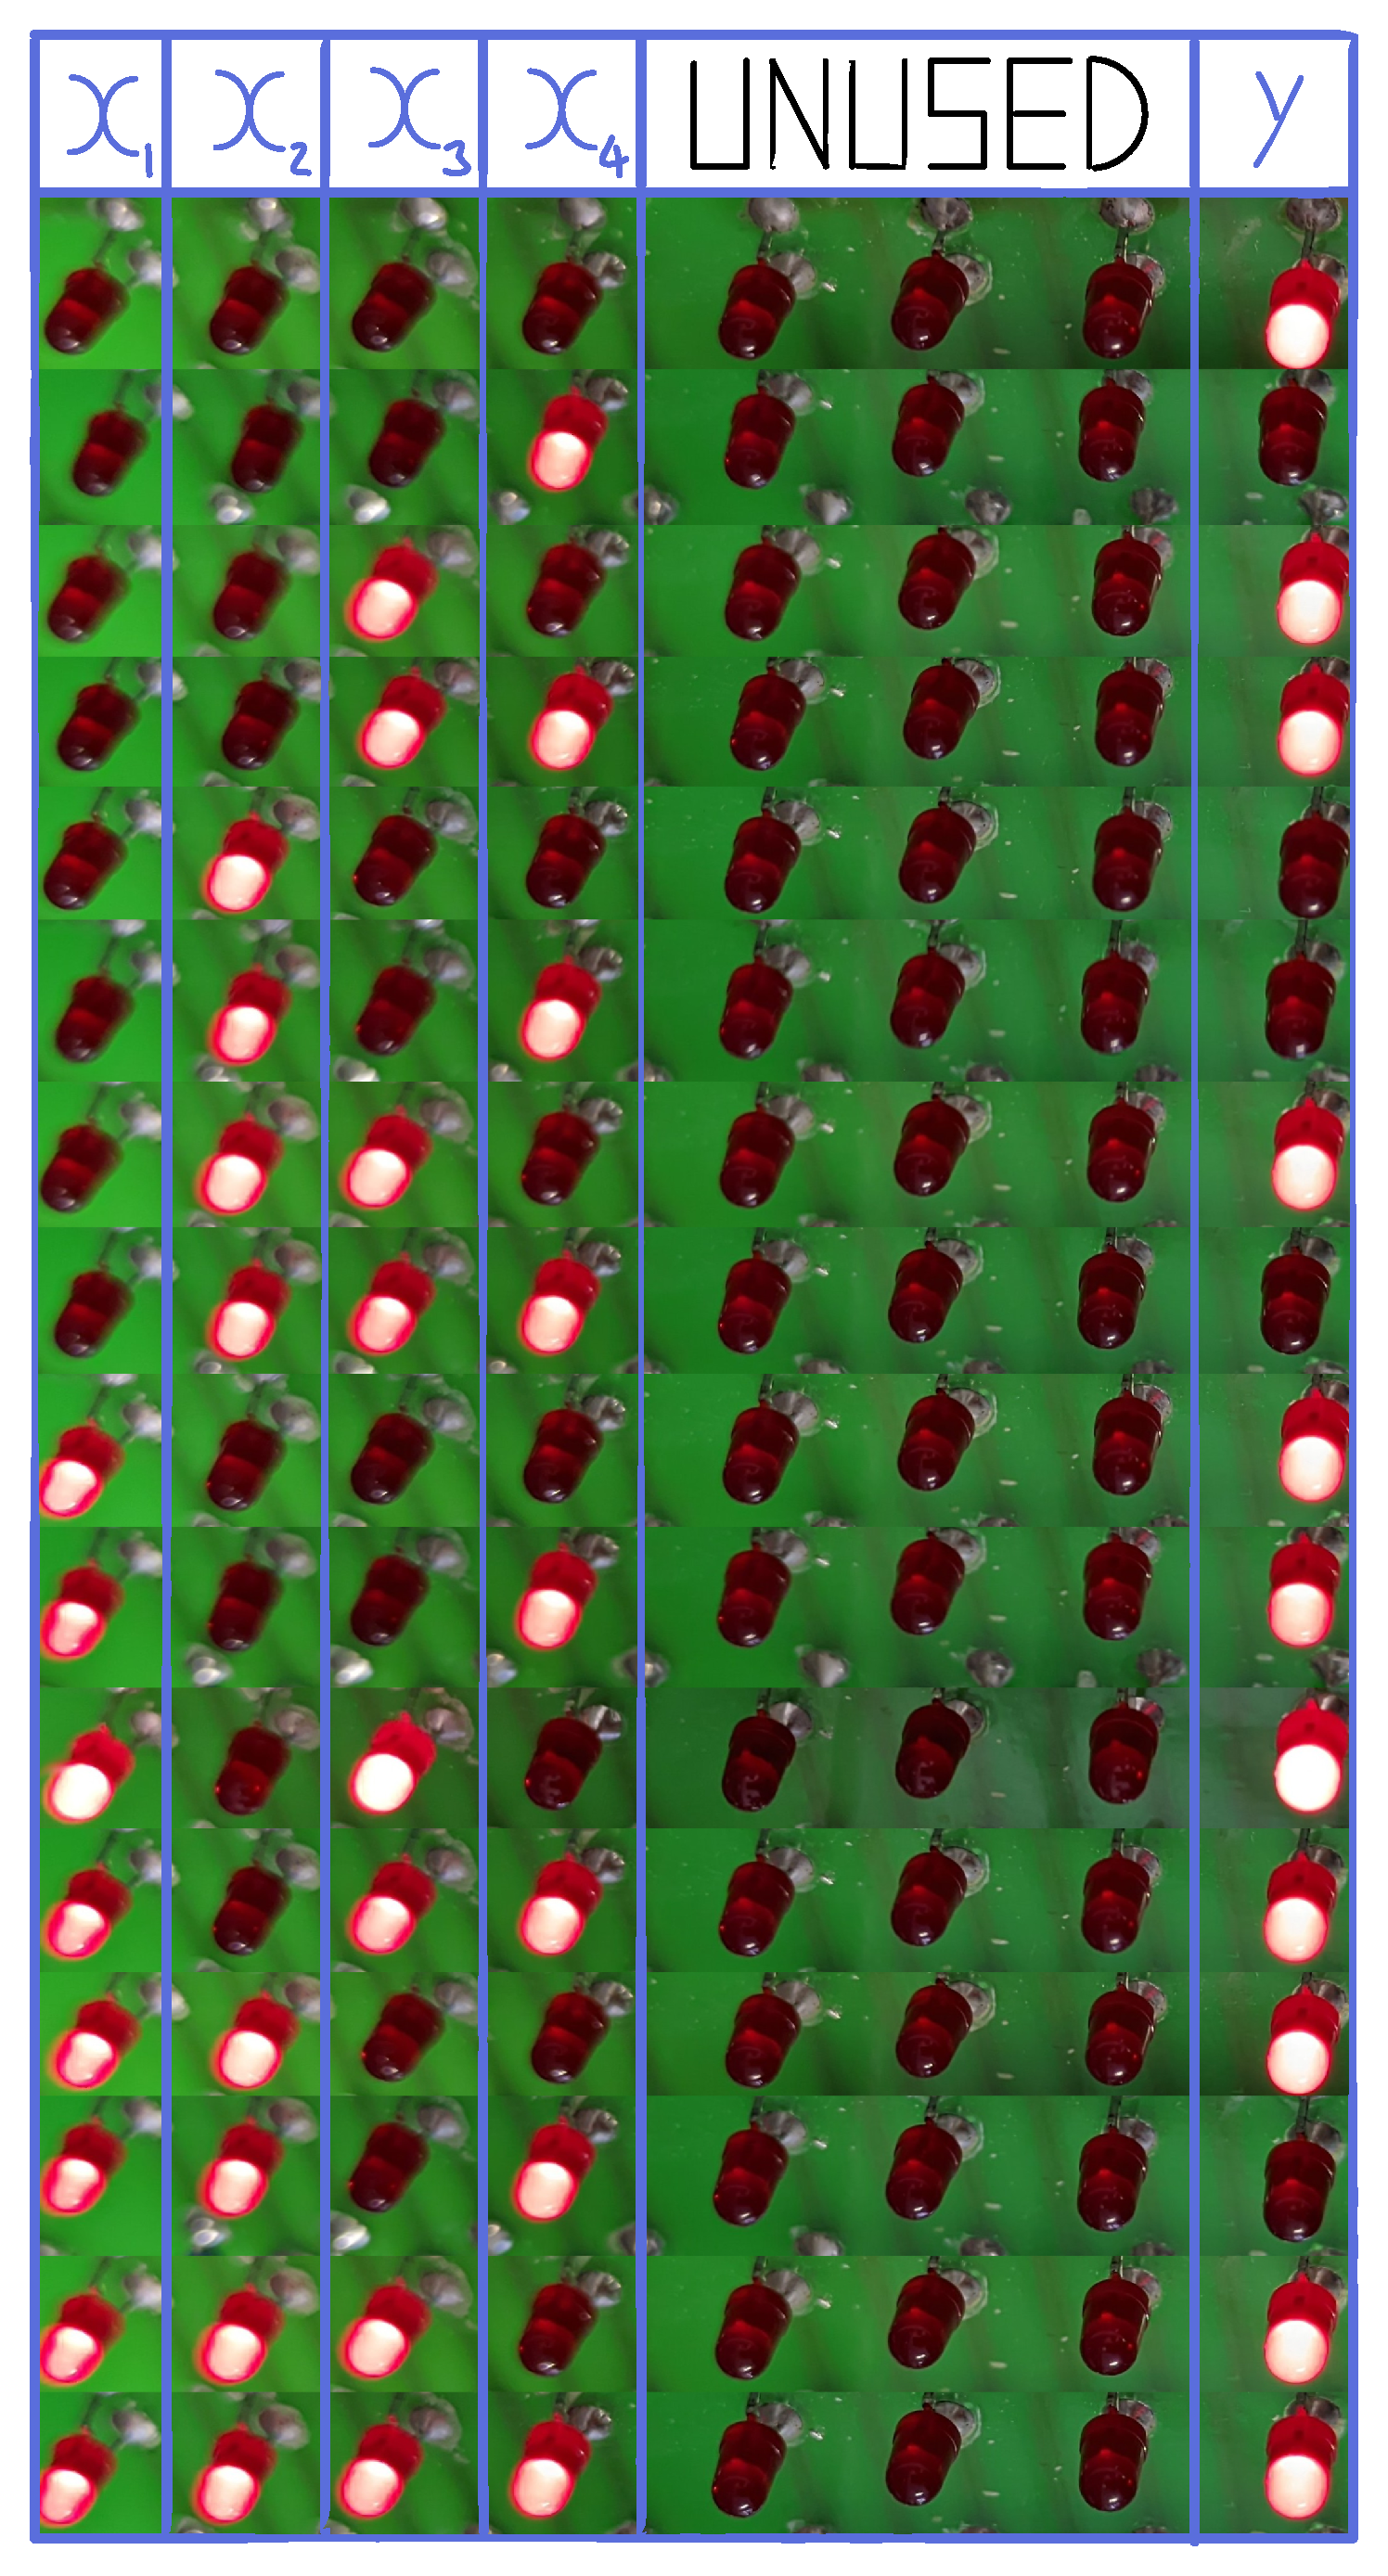
\includegraphics[width=0.95\textwidth,height=15cm]{./figures/messungen/WahrheitstabelleAlarm.pdf}
  \caption{}
  \label{fig:mess_wahrheitstabelle_alarm}
\end{figure}

Für die Untersuchung des Master-Switches im ausgeschalteten Zustand wurden die
eine zuvor wahre Eingangssignalkombination geschaltet und geschaut ob diese
nicht die Alarmanlage anschlagen lässt. Da die Schaltung zuvor, wie in
\autoref{fig:mess_wahrheitstabelle_alarm} ersichtlich, funktionierte ist
dadurch die Funktionstüchtigkeit des Master-Switches gezeigt.

% 2.3
% Die Ergebnisse sind zu protokollieren und zu diskutieren.

% zu 4: Auswertung siehe EPM Skript nur Besprechung von Umformungen und 
% Sachen die man mit den Messungen machen muss damit man Conclusion und Wissen 
% gewinnen kann.
% Entsprechend der in Punkt 2. angegebenen Beziehungen (Formeln) ist aus den
% Messergebnissen in Punkt 5. das in Punkt 1. formulierte Endergebnis zu
% berechnen. Oft ist eine Ermittlung des Endergebnisses aus einer grafischen
% Darstellung bzw. eine grafische Veranschaulichung zweckmaßig. Dabei kann
% die Verwendung von Millimeterpapier oder Computerprogrammen hilfreich sein.
% Wenn eine Bearbeitung der Daten auf dem Computer erfolgt, sollte bei der
% Darstellung der Graphen eine sinnvolle Skalenteilung des Koordinatensystems
% gemacht werden. Die Unsicherheitsbetrachtung f ̈ur die angegebenen Messwerte,
% sowie fur Zwischen- und Endergebnisse ist in diesem Abschnitt
% nachvollziehbar zu beschreiben. Dabei ist nach Kapitel 1 vorzugehen und
% insbesondere auf die Klassifizierung der Unsicherheit (Typ-A/B) und die
% Unsicherheitsfortpflanzung einzugehen.
\section{Auswertung}\label{sec:Auswertung}


% zu 5: Diskussion und Zusammenfassung
% In der Zusammenfassung stehen noch einmal die wichtigsten Messergebnisse, wobei auf Tabellen und
% Abbildungen nur verwiesen werden soll. Die Ergebnisse sind auch zu diskutieren. Insbesondere müssen
% Abweichungen zwischen Simulation und praktischer Durchführung diskutiert werden.
\section{Diskussion und Zusammenfassung}\label{sec:Diskussion} 
\subsection{Diskussion}


%Es wäre wohl vernünftiger gewesen, die Schaltung an der Steckplatine zunächst aufzubauen, um etwaige 
%Ungenauigkeiten durch die Widerstände 
\subsection{Zusammenfassung}

\newpage

\printbibliography

\listoffigures

\listoftables



\end{document}

